\documentclass[14pt,a4paper,report]{report}
\usepackage[a4paper, mag=1000, left=2.5cm, right=1cm, top=2cm, bottom=2cm, headsep=0.7cm, footskip=1cm]{geometry}
\usepackage[utf8]{inputenc}
\usepackage[english,russian]{babel}
\usepackage{indentfirst}
\usepackage[dvipsnames]{xcolor}
\usepackage[colorlinks]{hyperref}
\usepackage{listings} 
\usepackage{fancyhdr}
\usepackage{caption}
\usepackage{amsmath}
\usepackage{latexsym}
\usepackage{graphicx}
\usepackage{amsmath}
\hypersetup{
	colorlinks = true,
	linkcolor  = black
}

\usepackage{titlesec}
\titleformat{\chapter}
{\Large\bfseries} % format
{}                % label
{0pt}             % sep
{\huge}           % before-code


\DeclareCaptionFont{white}{\color{white}} 

% Listing description
\usepackage{listings} 
\DeclareCaptionFormat{listing}{\colorbox{gray}{\parbox{\textwidth}{#1#2#3}}}
\captionsetup[lstlisting]{format=listing,labelfont=white,textfont=white}
\lstset{ 
	% Listing settings
	inputencoding = utf8,			
	extendedchars = \true, 
	keepspaces = true, 			  	 % Поддержка кириллицы и пробелов в комментариях
	language = Matlab,            	 	 % Язык программирования (для подсветки)
	basicstyle = \small\sffamily, 	 % Размер и начертание шрифта для подсветки кода
	numbers = left,               	 % Где поставить нумерацию строк (слева\справа)
	numberstyle = \tiny,          	 % Размер шрифта для номеров строк
	stepnumber = 1,               	 % Размер шага между двумя номерами строк
	numbersep = 5pt,              	 % Как далеко отстоят номера строк от подсвечиваемого кода
	backgroundcolor = \color{white}, % Цвет фона подсветки - используем \usepackage{color}
	showspaces = false,           	 % Показывать или нет пробелы специальными отступами
	showstringspaces = false,    	 % Показывать или нет пробелы в строках
	showtabs = false,           	 % Показывать или нет табуляцию в строках
	frame = single,              	 % Рисовать рамку вокруг кода
	tabsize = 2,                  	 % Размер табуляции по умолчанию равен 2 пробелам
	captionpos = t,             	 % Позиция заголовка вверху [t] или внизу [b] 
	breaklines = true,           	 % Автоматически переносить строки (да\нет)
	breakatwhitespace = false,   	 % Переносить строки только если есть пробел
	escapeinside = {\%*}{*)}      	 % Если нужно добавить комментарии в коде
}

\begin{document}

\def\contentsname{Содержание}

% Titlepage
\begin{titlepage}
	\begin{center}
		\textsc{Санкт-Петербургский Политехнический 
			Университет Петра Великого\\[5mm]
			Кафедра компьютерных систем и программных технологий}
		
		\vfill
		
		\textbf{Отчёт по лабораторной работе №4\\[3mm]
			Курс: «Теория автоматического управления»\\[3mm]
			Тема: «Синтез управляющего устройства»\\[35mm]
			}
	\end{center}
	
	\hfill
	\begin{minipage}{.5\textwidth}
		Выполнил студент:\\[2mm] 
		Бояркин Никита Сергеевич\\
		Группа: 43501/3\\[5mm]
		
		Проверил:\\[2mm] 
		Нестеров Сергей Александрович
	\end{minipage}
	\vfill
	\begin{center}
		Санкт-Петербург\\ \the\year\ г.
	\end{center}
\end{titlepage}

% Contents
\tableofcontents
\clearpage

\chapter{Лабораторная работа №4}

\section{Цель работы}

Научиться синтезировать оптимальные управляющие устройства.

\section{Программа работы}

\begin{itemize}
	\item Синтезировать оптимальное управляющее устройство при условии полной измеряемости переменных объекта и полной управляемости системы. В качестве критерия оптимальности использовать интегральный критерий:
	
	$\int_{0}^{\infty}(\begin{bmatrix}
	x & x' 
	\end{bmatrix}Q\begin{bmatrix}
	x \\
	x' 
	\end{bmatrix}+RU^2)dt
	$, где $R=E=\begin{bmatrix}
	1 & 0 \\
	0 & 1 
	\end{bmatrix}, Q=\begin{bmatrix}
	\alpha & 0 \\
	0 & \beta 
	\end{bmatrix}$
	
	Структура управляющего устройства описывается уравнением:

	$U=-k_0x-k_1x'+gV$
	
	\item Проанализировать влияние параметров a и b (матрицы Q) на коэффициенты регулятора и показатели качества.
	\item Промоделировать работу системы при оптимальных параметрах регулятора.
\end{itemize}

\section{Индивидуальное задание}

$
\\
y''+25y'=5u'+25u, y(0)=0, y'(0)=0, u=1(t)\\\\
W(p)=\frac{y}{u}=\frac{5p+25}{p^2+25p} \\
$

$A=
	\begin{bmatrix}
	0 & 1 \\
	0 & -25 \\
	\end{bmatrix}
	, B=
	\begin{bmatrix}
	0 \\
	1 \\
	\end{bmatrix}
	, C=
	\begin{bmatrix}
	25 & 5 \\
	\end{bmatrix}
	$
	
\begin{figure}[h!]
	\centering
	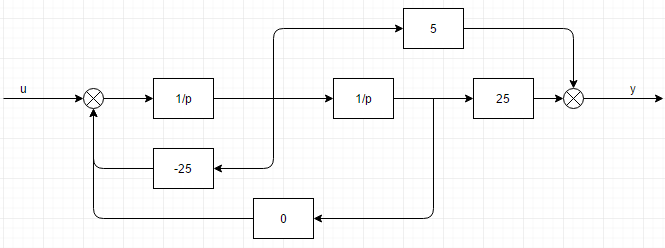
\includegraphics[scale = 0.73]{images/nfu.png}
	\caption{Структурная схема НФУ}
	\label{image:1}
\end{figure}	

\clearpage

\section{Ход работы}

\subsection{Подключение управляющего устройства}

При подключении управляющего устройства со структурой $U=-k_0x-k_1x'+gV$ получим, предполагая что $x_2=x', x_1=x$:

\begin{figure}[h!]
	\centering
	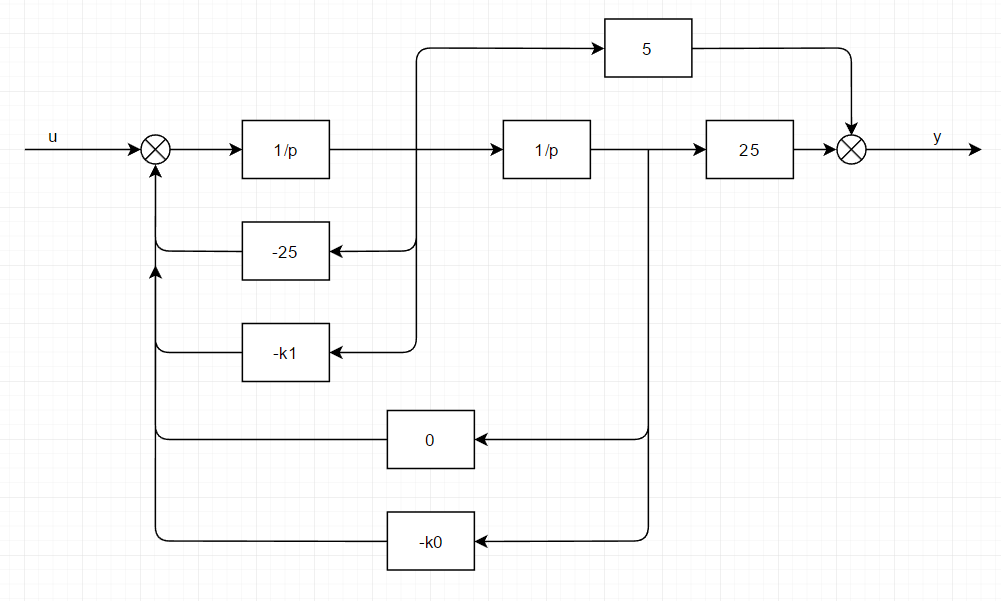
\includegraphics[scale = 0.60]{images/uunfu.png}
	\caption{Система с подключённым управляющим устройством}
	\label{image:2}
\end{figure}	

Составим передаточную функцию результирующей системы:

$W(p)=g\cdot W_1(p)\cdot W_2(p)=g\cdot \frac{5p+25}{p^2+(25+k_1)p+k_0}$

Характеристический полином результирующей системы:

$D(p)=p^2+(25+k_1)p+k_0$

\subsection{Определение области устойчивости}

Согласно критерию Гурвица для систем второго порядка, для устойчивости необходимо и достаточно, чтобы коэффициенты характеристического полинома были положительны, следовательно:

\begin{equation*}
\begin{cases}
	\text{$k_0>0$} \\
	\text{$k_1>-25$}
\end{cases}
\end{equation*}

\subsection{Нахождение коэффициента обратной связи}

Синтезируем устройство, оптимальное по интегральному критерию:

$\int_{0}^{\infty}(\begin{bmatrix}
x & x' 
\end{bmatrix}Q\begin{bmatrix}
x \\
x' 
\end{bmatrix}+RU^2)dt
$, где $R=E=\begin{bmatrix}
1 & 0 \\
0 & 1 
\end{bmatrix}, Q=\begin{bmatrix}
\alpha & 0 \\
0 & \beta 
\end{bmatrix}$

Воспользуемся уравнением Рикатти:

$A^TS+SA-(SB+N)R^{-1}(B^TS+N^T)+Q=0$, где $ S=\begin{bmatrix}
a & b \\
c & d 
\end{bmatrix}, R=E=\begin{bmatrix}
	1 & 0 \\
	0 & 1 
\end{bmatrix}, Q=\begin{bmatrix}
\alpha & 0 \\
0 & \beta 
\end{bmatrix}, N=\begin{bmatrix}
0 & 0 \\
0 & 0 
\end{bmatrix}$

Вычислим коэффициенты обратной связи при $Q=E$:

\begin{center}
	$\begin{bmatrix}
	0 & 1 \\
	0 & -25 \\
	\end{bmatrix}^T\begin{bmatrix}
	a & b \\
	c & d 
	\end{bmatrix}+\begin{bmatrix}
	a & b \\
	c & d 
	\end{bmatrix}\begin{bmatrix}
	0 & 1 \\
	0 & -25 \\
	\end{bmatrix}-(\begin{bmatrix}
	a & b \\
	c & d 
	\end{bmatrix}\begin{bmatrix}
	0 \\
	1 
	\end{bmatrix})\cdot(\begin{bmatrix}
	0 & 1
	\end{bmatrix}\begin{bmatrix}
	a & b \\
	c & d 
	\end{bmatrix})+\begin{bmatrix}
	1 & 0 \\
	0 & 1 
	\end{bmatrix}=\begin{bmatrix}
	0 & 0 \\
	0 & 0 
	\end{bmatrix}$
\end{center}

\begin{center}
	$
\begin{bmatrix}
1-bc & a-25b-bd \\
a-25c-cd & -d^2-50d+b+c+1 
\end{bmatrix}=\begin{bmatrix}
0 & 0 \\
0 & 0
\end{bmatrix}
$
\end{center}

Таким образом, при учете, что все элементы матрицы $S$ положительные:

\begin{equation*}
\begin{cases}
\text{$1-bc=0$} \\
\text{$a-25b-bd=0$} \\
\text{$a-25c-cd=0$} \\
\text{$-d^2-50d+b+c+1=0$} \\
\text{$a>0$} \\
\text{$b>0$} \\
\text{$c>0$} \\
\text{$d>0$} 
\end{cases}
\Longrightarrow
\begin{cases}
\text{$a=2\sqrt{157}$} \\
\text{$b=1$} \\
\text{$c=1$} \\
\text{$d=2\sqrt{157}-25$} 
\end{cases}
\end{equation*}

Таким образом, $S=\begin{bmatrix}
2\sqrt{157} & 1 \\
1 & 2\sqrt{157}-25 
\end{bmatrix}, K=B^TS=\begin{bmatrix} 1 & 2\sqrt{157}-25 \end{bmatrix}$. Данное решение удовлетворяет всем критериям устойчивости.

\subsection{Нахождение коэффициента масштабирования}

Чтобы вычислить коэффициент $g$, масштабирующий входной сигнал, воспользуемся тем, что в установившемся режиме выход системы будет определяться как $y=gV_0\cdot \frac{M}{M+1}$. Тогда при $g=\frac{M+1}{M}, y=V_0$, чего и требуется достичь.

Передаточная функция замкнутой системы:

$W_3(p)=\frac{B(p)}{B(p)+C(p)}=\frac{5p+25}{p^2+(25+k_1)p+k_0}$

Тогда:

$W_p(p)=\frac{B(p)}{C(p)}=\frac{5p+25}{p^2+(25+k_1)p+k_0-5p-25}=\frac{5p+25}{p^2+(20+k_1)p+(k_0-25)}$

Тогда:

$M=W_p(0)=\frac{25}{k_0-25}$

Для ранее вычисленных значений:

$K=\begin{bmatrix} 1 & 2\sqrt{157}-25 \end{bmatrix}, M=-\frac{25}{24}, g=\frac{1}{25}$

\clearpage

\subsection{Изучение влияния весовых коэффициентов на характеристики системы}

Исследуем, как изменение элементов весовой матрицы Q влияет на результирующие коэффициенты регулятора и на качество системы. Для этого будем решать уравнение Риккати для различных значений элементов матрицы Q.

\begin{center}
	$Q=\begin{bmatrix} \alpha & 0 \\
	0 & \beta \end{bmatrix} $
\end{center}
	
Выведем три типа зависимостей:

\begin{itemize}
	\item В зависимости от $\alpha$, где $\beta=1$.
	\item В зависимости от $\beta$, где $\alpha=1$.
	\item В зависимости от $\alpha$ и $\beta$ одновременно, где $\alpha=\beta$.
\end{itemize}

\subsubsection{Изучение влияния весовых коэффициентов на параметры регулятора}

Получим следующие зависимости параметров регулятора от коэффициентов:

\begin{figure}[h!]
	\centering
	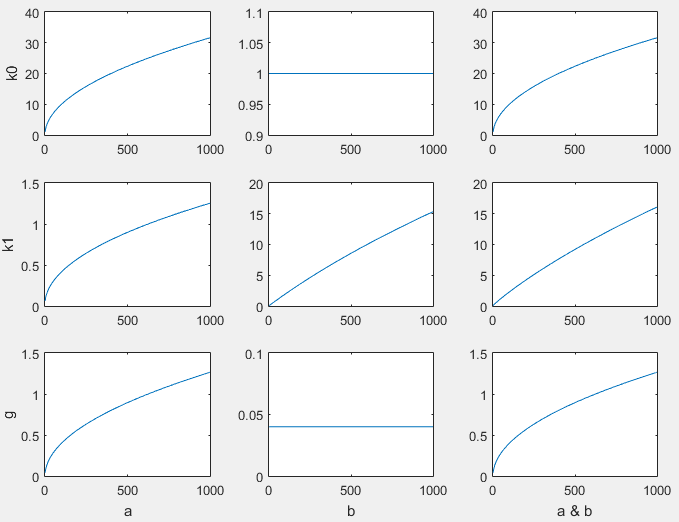
\includegraphics[scale = 0.85]{images/1.png}
	\label{image:3}
\end{figure}

По полученным данным можно заключить, что с увеличением параметра $\alpha$ также увеличиваются коэффициенты $k_0, k_1, g$, в то время как параметр $\beta$ увеличивает только коэффициент $k_1$, однако, делает это намного быстрее, чем $\alpha$.

\subsubsection{Изучение влияния весовых коэффициентов на качество системы}

Аналогично изучим влияние весовых коэффициентов на показатели качества. Будем оценивать его по корневым критериям - среднему геометрическому корней характеристического полинома и степени устойчивости (минимальный модуль вещественной части корней).

Оценим колебательность системы аналитически:

$D(p)=p^2+(25+k_1)p+k_0$\\

$p_{12}=\frac{-25-k_1\pm \sqrt{(25+k_1)^2-4k_0}}{2}$

Таким образом, можно считать, что комплексных корней не возникает, так как обычно коэффициент $k_0$ увеличивается вместе с $k_1$.

Построим зависимости весовых коэффициентов от корневых показателей качества:

\begin{figure}[h!]
	\centering
	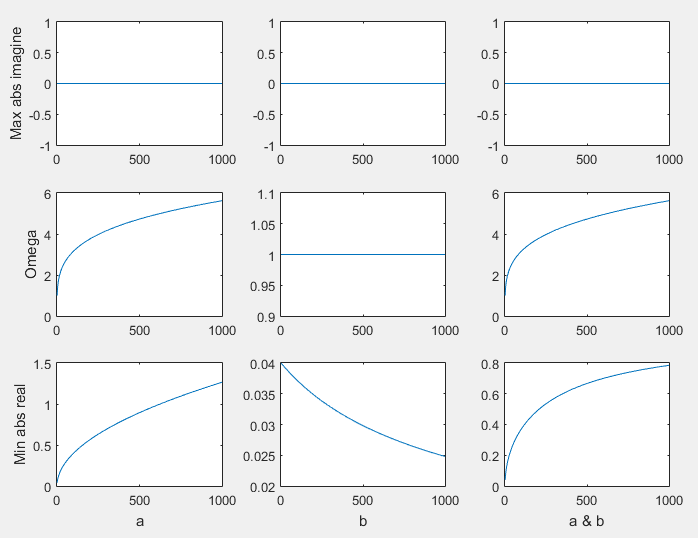
\includegraphics[scale = 0.85]{images/2.png}
	\label{image:4}
\end{figure}

Как и ожидалось, с увеличением весовых коэффициентов  матрицы Q, мнимые части корней равнялись нулю, что означает, что система не имеет колебательности. На показатель быстродействия наилучшим образом влияет параметр $\alpha$, однако он также негативно влияет на степень устойчивости. Единственной характеристикой, на которую благоприятно влияет параметр $\beta$ является степень устойчивости. 

Таким образом, можно компенсировать недостатки от увеличения параметра $\alpha$ одновременным увеличением параметра $\beta$. Если увеличивать их одновременно, возрастает быстродействие системы, а отклонение вещественных частей корней от мнимой оси возрастает незначительно и имеет верхнюю границу.

В общем случае рекомендуется увеличивать параметры $\alpha$ и $\beta$ одновременно, а для обеспечения необходимого уровня степени устойчивости сохранять соотношение $\beta>\alpha$.

\clearpage

\subsection{Моделирование работы системы}

Смоделируем систему при:

$Q=\begin{bmatrix}
1000 & 0 \\
0 & 1000 
\end{bmatrix}, k_0=31.6228, k_1=16.0883, q=1.2649$

\begin{figure}[h!]
	\centering
	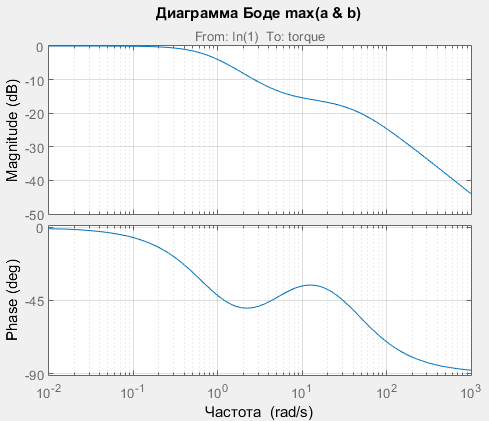
\includegraphics[scale = 0.70]{images/3.png}
	\caption{Диаграмма Боде}
	\label{image:5}
\end{figure}

\begin{figure}[h!]
	\centering
	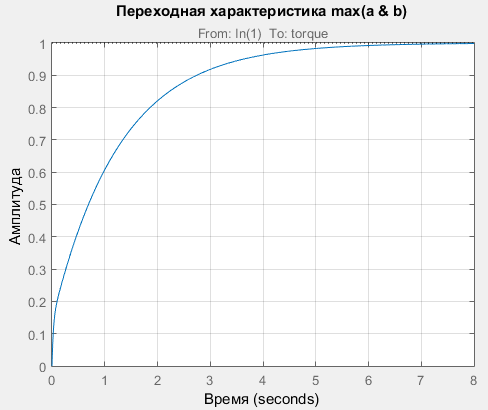
\includegraphics[scale = 0.70]{images/4.png}
	\caption{Переходная характеристика}
	\label{image:6}
\end{figure}

Увеличение быстродействия действительно заметно: для выбранных параметров установление процесса происходит примерно за 6 секунд, в то время как при $Q=\begin{bmatrix}
1 & 0 \\
0 & 1000 
\end{bmatrix}$ установление процесса происходит за 250 секунд.

\section{Вывод}

При условии полной наблюдаемости системы регулятор может быть реализован через обратную связь от переменных пространства состояния. Результирующая система может быть путём структурных преобразований представлена в виде системы с обратной связью, что позволяет применить для неё весь математический аппарат, рассмотренный в предыдущих работах.

Для линейных стационарных систем оптимальное решение может быть найдено путём решения матричного уравнения Риккати. Оно связывает матрицы системы и оптимальные коэффициенты для управления вида $U=-KX$. В качестве показателя оптимальности используется интегральный критерий.

Для различных значений параметров $\alpha$ и $\beta$ матрицы $Q$ было экспериментально доказано, что с ростом обоих параметров одновременно корневые критерии качества увеличиваются (или незначительно уменьшаются в случае со степенью устойчивости). В случае, если степень устойчивости является критической, должно сохраняться соотношение $\beta>\alpha$, если критично быстродействие, то $\beta<\alpha$.

\end{document}